\subsection{Glass Tile}
\paragraph{Korrektheit}
Die Korrektheit der Implementierung des portierten Algorithmus wurde mithilfe der Gegl-Testumgebung geprüft mit dem Ergebnis, dass für verschieden gewählte Parameter stets eine Übereinstimmung mit dem GIMP-Referenzbild besteht.

\paragraph{Laufzeit}
Das Testsystem ist ein Intel Core-2-Duo 2,2 GHz Notebook mit zwei Kernen, 2GB RAM und Linux Ubuntu 13.04 64-bit als Betriebsystem. Als Testbild wurde ein 5000x3450 Pixel großes png-Bild mit 21 MB Dateigröße verwendet. Als Umgebungsvariablen für Gegl wurden die Default-Werte verwendet und die Parameter des Filters für Breite und Höhe der Kacheln waren jeweils 47 Pixel. Es wurden jeweils 50 Testläufe durchgeführt, sowohl für die sequentielle Version, als auch für ein bzw. zwei Threads in der parallelen Version. Die Ergebnisse werden in Abbildung~\ref{fig:gtile-runs} aufgezeigt. Man sieht, dass die parallele Version etwas schlechter abschneidet als die sequentielle. Die Parallelisierung dieses Filters lohnt sich demnach nicht.

\begin{figure}[h]
\begin{center}
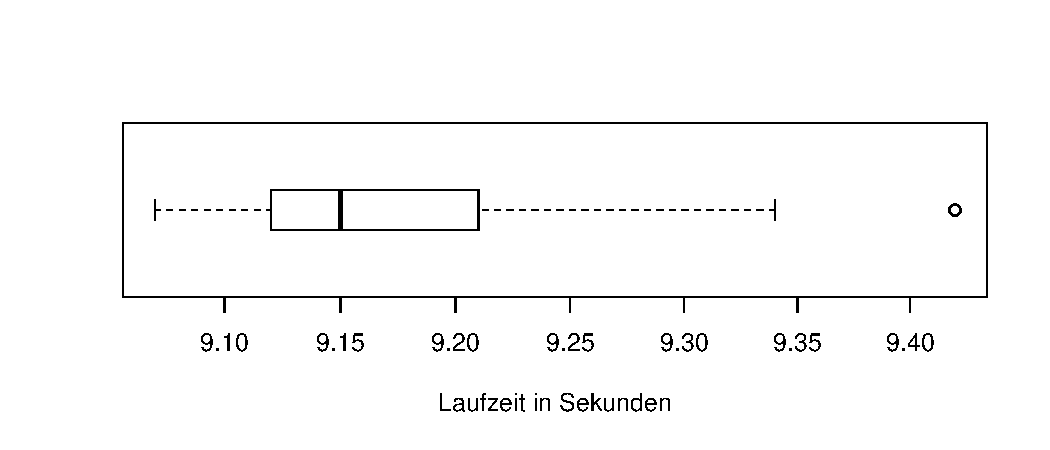
\includegraphics[width=1.0\textwidth]{graphs/glass-tile_seq.pdf}\newline
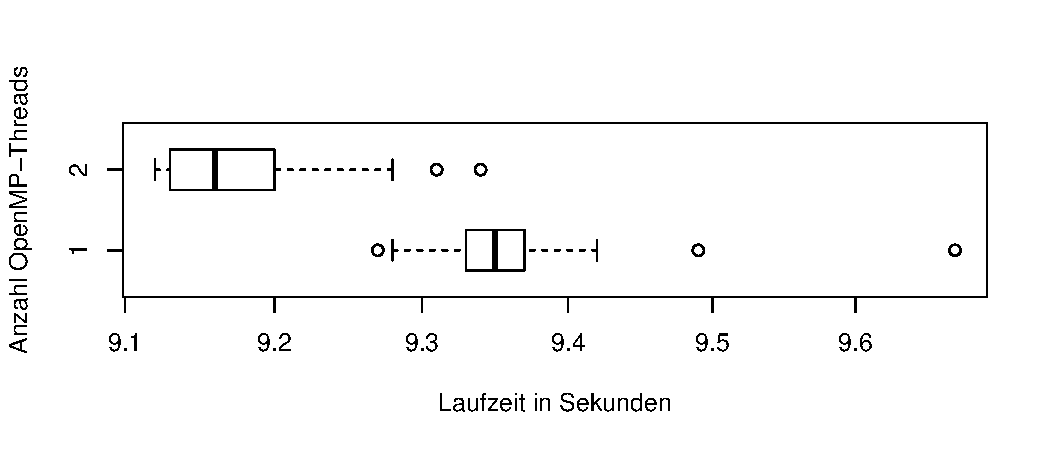
\includegraphics[width=1.0\textwidth]{graphs/glass-tile_2threads.pdf}
\end{center}
\caption{Laufzeit von Glass Tile (sequ. Variante oben, parallele Variante unten)}\label{fig:gtile-runs}
\end{figure}

Für die exemplarische detaillierte Ansicht der einzelnen Gegl-Aufrufe und die zugehörige Zeitmessung wurde jeweils ein Aufruf gemacht, bei dem \emph{GEGL-DEBUG-TIME} auf \emph{TRUE} gesetzt war. Wie in Abbildung~\ref{fig:gtile-dias} zu sehen ist, macht die eigentliche Operation nur einen Bruchteil der Gesamtzeit aus und die parallele Version benötigt länger als die sequentielle Version, was bereits weiter oben angedeutet wurde. Die sequentielle Variante gegl:tile-glass-seq wird in 0,73 sek ausgeführt, wohingegen die parallele Version mit 2 Threads gegl:tile-glass in 0,85 sek läuft.

\begin{figure}[h]
\begin{center}
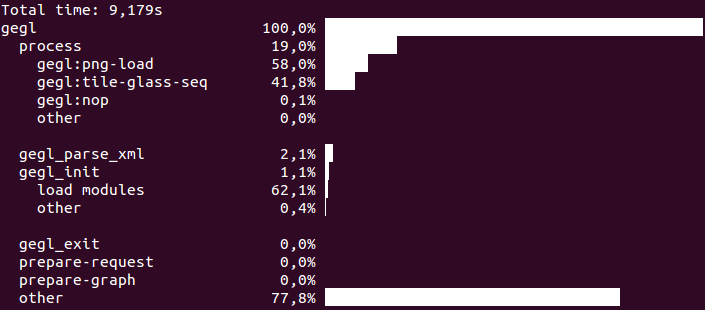
\includegraphics[width=1.0\textwidth]{gtile_seq_dia.png}
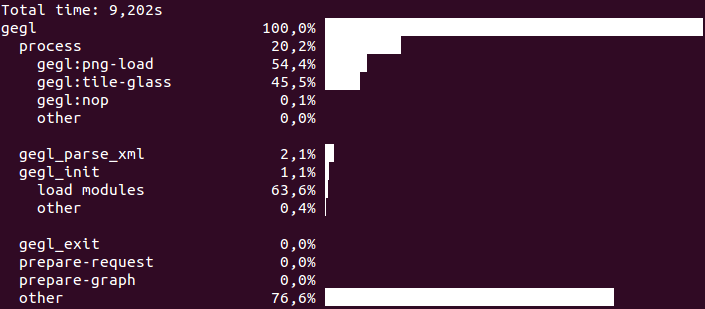
\includegraphics[width=1.0\textwidth]{gtile_par_dia.png}
\end{center}
\caption{Detailansicht der Gegl-Aufrufe (sequ. Variante oben, parallele Variante mit 2 Threads unten)}\label{fig:gtile-dias}
\end{figure}
